\documentclass[12pt]{article}

\usepackage{cite}
\usepackage{listings}
\usepackage{times}
\usepackage{color}
\usepackage{url}
\usepackage{multirow}
\usepackage{enumitem} % Use for enumerating A, B, C etc...
\urlstyle{same} % Used for formatting formatting url footnotes
\usepackage{fancyhdr} % Header
%\usepackage[table]{xcolor}% http://ctan.org/pkg/xcolor
\usepackage[table,xcdraw]{xcolor}
\usepackage{soul} % highlighting
%\usepackage{pgfgantt} % Project timeline
\usepackage[titletoc,toc,title]{appendix} % Need for appendix, page numbering
\usepackage{tikz}
\usetikzlibrary{calc,arrows.meta,fit,positioning}
%\usepackage{amssymb,graphicx} % Events and milestones
\usepackage{amsmath}
\usepackage{mathtools}
\usepackage{bbm}
\usepackage{amssymb}
\usepackage{booktabs} % used for \toprule in tables
\usepackage{wrapfig,booktabs} % Wrap text around table
\usepackage{booktabs} % used for \toprule in tables
\usepackage[table,xcdraw]{xcolor}
\DeclarePairedDelimiter\ceil{\lceil}{\rceil}
\DeclarePairedDelimiter\floor{\lfloor}{\rfloor}      
\usepackage[final]{pdfpages}
\usepackage{tocloft} % Table of contents spacing
\usepackage{xcolor,colortbl} %%% Color Table Header

\usepackage{makecell}

%\usepackage{subcaption} % Side by side images
%\usepackage{pgfplots} % Bar chart. Graph

\usepackage{xspace} % Needed for et al.
%\newcommand{\etal}{{et al.\@\xspace}} 
\newcommand{\etal}{\emph{et~al.}\xspace} 

\usepackage[bottom=1in, left=1in, right=1in, top=1in]{geometry} 


\usepackage[english]{babel}
\usepackage[utf8x]{inputenc}
\usepackage{graphicx}
\usepackage{wrapfig}
%\usepackage{lipsum}
%\usepackage{pgfgantt}

%\usepackage{minted} % Side by side code




\newcommand{\todo}[1]{\textcolor{cyan}{\textbf{[#1]}}}
\newcommand{\dan}[1]{\textcolor{blue}{{\it [Dan says: #1]}}}
\newcommand{\qi}[1]{\textcolor{red}{{\it [Qi says: #1]}}}
\newcommand{\sakshi}[1]{\textcolor{green}{{\it [Sakshi says: #1]}}}


%%% Start column formatting
% Note: In overleaf sometimes columns fail to render. Check on PDF Output
\newcolumntype{L}[1]{>{\raggedright\arraybackslash}m{#1}} % raggedright= align left
\definecolor{Gray}{gray}{0.80} % the lower the #, the darker it gets
%%% End Table formatting

%%%% Start toggling showing/hiding some information
\newif\ifShowAll
\ShowAlltrue % Display All Info
%\ShowAllfalse % Hide Some Info


\newcommand{\Title}{Applying Dynamic Bayesian Matrix Factorization to Predict Tactic Volatility in Self-Adaptive Systems}

\newcommand{\shortTitle}{Dynamic Bayesian Matrix Factorization to Predict Tactic Volatility} % Used in the heading just so it fits



\newcommand{\CallNumber}{BAA N00174-18-0001}
\newcommand{\CallName}{XXXX}

\usepackage{fancyhdr} % Header
\pagestyle{fancy}
\lhead{Krutz (RIT)}
%\lhead{\shortTitle}
%\rhead{}
\rhead{\emph{\shortTitle}}


\usepackage{lastpage}




\setlength\cftparskip{-.7pt} %% Table of contents spacing
%\setlength\cftbeforechapskip{0pt}

\begin{document}

\begin{titlepage}

\newcommand{\HRule}{\rule{\linewidth}{0.3mm}} % Defines a new command for the horizontal lines, change thickness here

%%%%%%% Start new Title format


%% DK: I am not sure if we should have this
%\noindent\large \CallName, \CallNumber\\[.20cm] % Call Name

\noindent\large \CallNumber\\[.20cm] % Call Name


\noindent \LARGE \textbf{\Title}\\[.10cm] % Title

\noindent \large  \underline{\textbf{Technical Proposal}}\\ [.15cm] 

\begin{tabular}{ L{50mm} L{100mm} }

%\normalsize \textbf{Technical Proposal:} & \normalsize  \CallName, \CallNumber  \\

%\noindent\large Technical Proposal: N00174-18-0001\\[.20cm]
%\noindent\large NEC Technical POC: \\[.20cm]
%\noindent\large Topic Number: \\[.20cm]

\normalsize \textbf{BAA Number:} & \normalsize  N00174-18-0001  \\


% Charlotte George NSWCCD Carderock Division
% technical lead for CD-03, Dr. Christopher Kent

\normalsize \textbf{Topic Number:} & \normalsize  CD-03  \\ 
\normalsize \textbf{NEEC Technical POC:} & \normalsize  Ms. Charlotte George (NSWCCD Carderock Division)  \\
 & \normalsize  Email: charlotte.george@navy.mil  \\
 & \normalsize  Phone: (301) 227-8869  \\


% Bio on Charlotte: https://www.navsea.navy.mil/Portals/103/Documents/NSWC_Carderock/Waves-Issue3_2017_web.pdf?ver=2017-10-31-155747-633

\vspace{-0mm} \normalsize \textbf{NEEC Technical Lead:} & \normalsize  Dr. Christopher Kent  \\
 & \normalsize Email: christopher.p.kent1@navy.mil  \\


\normalsize  \\ % Just add a space 
\normalsize \textbf{Organization:} & \normalsize  Rochester Institute of Technology  \\
\normalsize \textbf{Technical POC/PI:} & \normalsize  Dr. Daniel Krutz \\
 & \vspace{-2mm} \normalsize Department of Software Engineering
 \\
 
   & \vspace{-4mm} \normalsize 152 Lomb Memorial Drive \\
   & \vspace{-6mm} \normalsize Rochester, NY 14623 \\
   & \vspace{-8mm} \normalsize Phone: (585) 475-2896 \\
   & \vspace{-10mm} \normalsize Email: dxkvse@rit.edu \\
     

 \vspace{-8mm}    \normalsize \textbf{Period of Performance:} &  \vspace{-8mm} \normalsize Year 1: Feb 1 2019 - Jan 30, 2020 \\
 &  \vspace{-9mm} \normalsize Year 2: Feb 1 2020 - Jan 30, 2021 \\
  &  \vspace{-11mm} \normalsize Year 3: Feb 1 2021 - Jan 30, 2022 \\
  
%  \vspace{-8mm}    \normalsize \textbf{Total funds requested:} &  \vspace{-8mm} \normalsize Year 1: \$XX \\
% &  \vspace{-9mm} \normalsize Year 2: \$XX \\
% &  \vspace{-11mm} \normalsize Year 3: \$XX } \\

\end{tabular}



% (1) Nine months (15 December 2018 through 30 September 2019) 
% (2) Twelve months (01 October 2019 through 30 September 2020) 
% (3) Three months (01 October 2020 through 14 December 2020)


% 15 December 2018 through 30 September 2019

 \end{titlepage}

\cfoot{\thepage}
\pagenumbering{alph} % Start roman numbering
\setcounter{tocdepth}{1} % Show sections

\cfoot{} % Leave blank

% https://texblog.org/2013/04/29/latex-table-of-contents-list-of-figurestables-and-some-customizations/


%\tableofcontents
%\addtocontents{toc}{~\hfill\textbf{Page}\par}
%\chapter{...}

\renewcommand\contentsname{Table of Contents}



\tableofcontents
%\vspace{-6mm}
\listoffigures
%\vspace{-4mm}
\listoftables
\newpage

\setcounter{page}{1}
\pagenumbering{arabic} % Switch to normal numbers

%\cfoot{\thepage\ of \pageref{LastPage}}
\fancyfoot[C]{Page~\thepage~of~\pageref{lastpage}}

\section{Technical Approach and Justification}
%%%%%%%%%%%%%%%%%%%%%%%%%%%%%%%%%%%%%%%%%%%%%%%%%%%%%%%

% Techniques for expanding autonomous operations in air, surface, and undersea domains. Consider concepts for autonomy architecture; autonomous command and control; applying artificial intelligence/machine learning; sensor integration and fusion; launch and recovery; platform design and manufacturing; and lightweight/long endurance power and propulsion systems.
 
% DK: Clear this up
This project aims to develop a dynamic Bayesian matrix factorization framework to predict tactic volatility in self-adaptive/autonomous systems. The proposed framework will enable autonomous systems to better account for uncertainty and tactic volatility allowing them to be more \ul{resilient, efficient, effective at anticipating bad and erratic decisions, and support the completion of mission and system critical operations}. This will be accomplished in {\em XXXX innovative and integrated ways to maximize the overall effectiveness of complex decision-making}: (1) to analyze\todo{.......} % DK: Update with the tasks that we identify. Probably stick with 2 or so for this project

% Analyze heterogeneous data to predict tactic volatility
% 



% An action primitive that produces a change in the system, leaving it in a consistent state [28].

% DK: Start describing tactics

\emph{Tactics} are actions performed by self-adaptive systems to respond to changes in their environment or to achieve system objectives. Example tactics include reducing non-essential functionality on an autonomous underwater vehicle (AUV) when battery levels are low or the provisioning of an additional virtual machine in a web farm when the workload reaches a specific threshold. The AI components in self-adaptive systems rely upon accurate information to select the tactic(s) that will lead to decisions that produce the maximum \emph{utility} (benefit). Inaccurate information used in the decision-making process will frequently lead to decisions producing less than optimal benefit, or even undesired outcomes. Unfortunately, most self-adaptive processes are limited in that they are unable to account for tactic volatility and assume that all tactic operations perpetually have static attributes. Additionally, no known techniques have the ability to properly anticipate tactic volatility. This inability to account for and anticipate tactic volatility creates uncertainty that can be severely detrimental to the self-adaptive process. A robust prediction mechanism is needed to enable self-adaptive systems to better anticipate and account for tactic volatility to reduce this uncertainty. \ul{This pioneering research will develop a dynamic Bayesian matrix factorization framework to support autonomous operations.} By enabling the system to more accurately account for tactic volatility, this innovative work will {\bf increase the system's resiliency, efficiency, and ability to complete mission critical operations.}

% likely going to make bad/erratic decisions. <- Likely add this in there


\vspace{-3mm}\paragraph{A Motivating Example} 
As a motivating example, we will use the scenario of an Autonomous Underwater Vehicle (AUV) encountering an obstacle. As shown in Figure~\ref{fig:AUVObstacleExample}, the AUV has has two options when encountering this barrier: Option \#1) AUV turns to avoid obstacle; Option \#2) AUV stops before hitting the obstacle. We will also assume that the AUV's \hl{tail rudder} has been operating incorrectly, meaning that its turning ability is hindered. Additionally, the AUV's `reverse' propeller mechanism enabling it to stop has been only operating at partial rotational speed, meaning that it will take longer to execute a `braking' action than originally anticipated. While it is system critical that the AUV avoid impacting the obstacle, a secondary goal is for the AUV to not stop and continue on its mission. Table~\ref{table:tacticVolatilityInfo} displays the volatility and the confidence level of each predicted tactic volatility value. In this scenario each tactic is anticipated to be able to lead to outcomes that avoid the obstacle. The primary differentiating factor between the two options is the confidence level of the predicted tactic volatility. \dan{clean this up}


%Table~\ref{table:tacticVolatilityInfo}


% DK: Not sure if we should mention something about the AUV rising

% In the described scenario, the  action would be for the AUV to turn to avoid the obstacle. Unfortunately, since the confidence level of the predicted tactic volatility is low, the optimal action would likely be for the AUV to performing a `braking' action due to its much higher confidence of the tactic. This would provide a higher amount of certainty that the AUV would avoid the obstacle. %and since it was much more likely to ensure that the system/mission critical operation of avoiding the barrier was achieved.

\begin{figure}[h]
	\centering
%    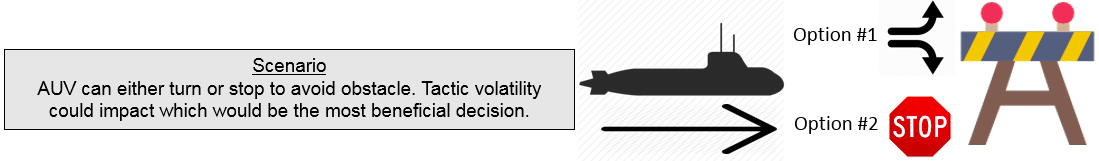
\includegraphics[scale=0.55]{images/AUVObstacle.png}
    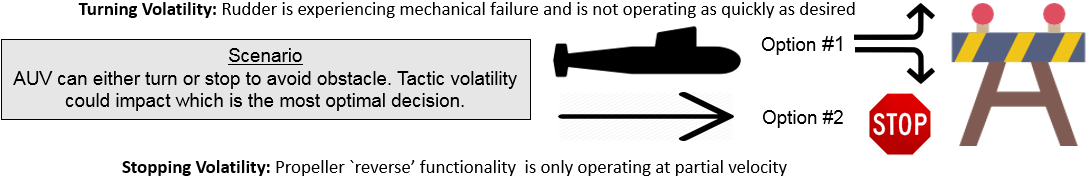
\includegraphics[scale=0.55]{images/AUVObstacle2.png}
    \caption{Example AUV Making a Decision That Could Be Impacted By Tactic Volatility\dan{?show confidence here}`}
    \label{fig:AUVObstacleExample}
\end{figure}

% ? Maybe change the obstacle to be a rock


%Table~\ref{table:tacticVolatilityInfo}

\begin{table}[h]
\begin{center}
\caption{Tactic Volatility in AUV Example}
\label{table:tacticVolatilityInfo}

\begin{tabular}{ |c|l|l|p{4.18cm}|l|p{2.05cm}| } 
 \hline
 \bfseries & \bfseries Action &  \bfseries AUV Component & \bfseries Observed Tactic Issue & \bfseries Impact & \bfseries Prediction ~~~Confidence  \\ \hline

 1 & Turn & Rudder & Rudder partially turning & Turn radius  & 50\% \\ \hline
 2 & Stop & Propeller `Reversing’ & Propeller `Reverse' is operating at partial speed & Stopping takes longer & 95\% \\ \hline


% `Reverse' on propeller is only operating at partial speed
% Propeller `Reversing’ & `Reverse' on propeller is only able to turn at partially desired rate & Stopping takes longer


   \end{tabular}
  \end{center}
\end{table}

% Can only turn at partially expected

%We will also assume that due to a system malfunction the AUV's rudders enabling it to turn have been operating slower than expected, meaning that it will taking longer to turn than anticipated.  Additionally, the AUV's `reverse' propeller mechanism enabling it to stop has been only operating at half strength, meaning that it will take longer to execute a `braking' action than originally anticipated.

%As a motivating example, we will use the scenario of an Autonomous Underwater Vehicle (AUV) encountering an obstacle. As shown in Figure~\ref{fig:AUVObstacleExample}, the AUV has has two options when encountering this barrier: I) Option \#1: AUV turns to avoid obstacle II) Option \#2: AUV stops before hitting the obstacle. We will assume that it is system-critical that the AUV avoids hitting the obstacle. We will also assume that due to a system malfunction the AUV's rudders enabling it to turn have been operating slower than expected, meaning that it will taking longer to turn than anticipated.  Additionally, the AUV's `reverse' propeller mechanism enabling it to stop has been only operating at half strength, meaning that it will take longer to execute a `braking' action than originally anticipated.

% Add in something about an uncertainty reduction tactic if we are going to use it?
% Bad/erractic decision
% Where is confidence level? - It should bre shown here


% Put these results into a table


In this scenario, we will assume that the predicted outcome of both tactics would lead to the AUV avoiding the barrier. The primary differentiating factor between the two tactic options is the significantly different confidence level of the predicted \hl{volatility}. Due to the higher confidence level of option \#2 (stopping), it is likely the better choice. Since it is system critical that the AUV avoid the barrier, it will likely be better for the AUV to go with the safer option even though it doesn't achieve the secondary benefit of not stopping.




%, even though it doesn't achieve the secondary benefit of not stopping.

%In the example, option \#2 (stopping) is likely the better choice. This is due to the confidence level of the predicted tactic volatility being much higher than the alternative (option \#1). Since it is system critical that the AUV avoid the barrier, it will likely be better for the AUV to go with the safer option, even though it doesn't achieve the secondary benefit of not stopping. \dan{I don't love how this is explained. It also needs to explain how each predicted volatility level will enable the system to meet its objective}

%This is the case even though a secondary goal of not stopping will not be achieved.



% After talking about how the system needs to account for this volatility, now talk about predicting this volatility is important

Tactic volatility should be factored into the decision-making process as it could substantially impact the most appropriate action for the AUV to take. In the provided scenario, when not properly accounting for observed tactic volatility the AUV could incorrectly assume that braking or turning actions were performing better than they actually were; thus potentially leading to the AUV hitting the obstacle. For example, the AUV could decide to start turning or braking operations too late, or could choose a tactic that was much more likely to lead to the AUV hitting the obstacle. A tactic volatility aware solution that is able to accurately predict this variability will reduce uncertainty in the decision-making process, and support the system in making the most optimal decision. Through our dynamic Bayesian matrix factorization process, we will enable the system to better anticipate this tactic volatility and therefore anticipate bad \& erratic functionality.

% Based on previously observed criteria, the AUV will need to determine which tactic(s) are most beneficial for ensuring that it does not hit the obstacle. Not accounting for previously experienced tactic volatility in the decision-making process will likely lead to a sub-optimal decision being selected, one that could potentially lead to catastrophic failures. Through our dynamic Bayesian matrix factorization process, we will enable the system to better anticipate this tactic volatility and therefore anticipate this bad/erratic functionality.


% DK: Will need to edit these based on what is actually used in our scenarios. 
% DK: I am also not sure if this should go here
\vspace{2mm}
Some of the forms of volatility that our \emph{Tactic Volatility Aware (TVA)} solution will enable system-adaptive systems to account for include:

  \begin{enumerate}[noitemsep]
    \item \textbf{Tactic Latency: }The amount of time required to implement a tactic is known as \emph{tactic latency}~\cite{Moreno:2018:FED:3208359.3149180,moreno2017adaptation}. Examples of tactic latency include the time required to activate a virtual machine in a cloud, or the time it takes a medical device to administer the dosage of a drug. This latency time can significantly vary between different tactics, and the volatility of these tactic latency times can also be quite diverse. The latency of each tactic may have a large impact on the decisions made by the system.
    
    \item \textbf{Tactic Dependability: }The measure of how well a tactic correctly produces its expected functionality is known as \emph{Tactic Dependability}. Due to numerous reasons, tactics can sometimes fail to produce the expected results. A tactic that performs a calculation could return an inaccurate result, or a virtual machine could fail to properly activate. Knowing when a tactic is not working dependably is imperative for an autonomous system.
    
    \item \textbf{Tactic Availability: }  Tactics may have different amounts of availability, which should be accounted for in the self-adaptive process. In a self-adaptive system with multiple options, the system may not always be aware of the availability of each option. For example, perhaps a tactic using a remote computer is only accessible 80\% of the time, but the only way to determine this is to try the tactic. The unavailability of this tactic should be factored into the determination process since trying unavailable tactics may incur resource costs. % DK: Might want to remove this as availability could be deemed to be the same as dependability
    
%    \item \textbf{XXXX} XXXX.


  \end{enumerate}




Accounting for tactic volatility will enable the system to:
%By accounting for this observed tactic volatility, will enable the system to:


% DK: I am not sure if this section should be moved
% Dk: Make sure that our process covers each of these
\begin{itemize}[noitemsep]

    
    % When mission/safety critical operations are being done, the best decision may be the safe one
    % Can be passed a maximum expected threshold
    % Can be generally factored into the decision-making process
    % 
    
    
    \item \textbf{Increase System Resiliency and Ability to Complete Critical Tasks: } Self-adaptive systems are frequently tasked with completing mission or critical operations. These could range from a medical device administering an essential drug, to a UAV engaging a target to assist troops in contact. The inability to sufficiently account for tactic volatility can have a profoundly adverse impact on the system's ability to complete safety/mission critical operations. By accounting for tactic volatility, the proposed process will enable the system to make more accurate and informed decisions; ones which lead to the increased ability to reliably execute safety/mission critical operations. 
    
    % DK: This one is a bit redundant with the others, but seems to be something the PM likes
    \item \textbf{Enable the system to predict bad and erratic decisions: }By creating accurate tactic predictions, the self-adaptive system will be able to anticipate decisions that are outside of the tolerated threshold, decisions with unacceptable amounts of volatility and other decisions that will lead to undesirable outcomes. 

    \item \textbf{Increase Decision-Making Efficiency: }Self-adaptive systems typically need to make fast, efficient decisions. By enabling the system to learn from observations, it will be able to make decisions that lead to greater system efficiency.

    \item \textbf{Assist with Concurrent and Subsequent Tactic Decisions: } Many self-adaptive systems are expected to decide upon and execute numerous concurrent tactics on a regular basis. This can become very complicated very quickly as tactics frequently do not occur in a silo and tactic decisions may impact concurrent and subsequent decisions. The proposed learning model will not only consider the impact of a potential decision on the specific tactic, but how it could impact concurrent and potential subsequent tactic decisions as well. 
    
 %   \item \textbf{Others: }XXXXX
    
\end{itemize}



%\todo{Why predicting volatility is important}  




% UAV is deciding upon something. 
%   Latency Volatility: How long until X is ready to do
%   Dependability Volatility: Will the operation return the expected benefit
%   Availability Volatility: Will the operation be ready to function as desired

%%%% Scenario


% A)
% Sub decides that it needs to turn
%   Avail: Rudders only work 50% of the time when tried
%   Dependability: Only turn 80% of the way
%   Latency: Take 3 seconds to work instead of the expected 4 seconds (worn out gears)

% > Should create a scenario where there are multiple options
%   Obstacle is detected
%   Option A: Sub will put on breaks
%   Option B: Sub will turn 




\vspace{2mm}

A robust process for predicting tactic volatility is imperative for a self-adaptive system to properly account for and anticipate real-world volatility. To address this challenge, this project provides a comprehensive machine learning framework to collectively address the following \underline{\bf unique challenges}, aiming to help autonomous systems {\bf improve their overall effectiveness in predicting and accounting for tactic volatility:} 

% DK: Update this on what we are actually doing with our process
% Dk: I am not sure some of these have anything to do with how we will be predicting volatility?
% DK: Much of this wording was taken from the ONR submission. We will need to check to see if it is still accurate or not
% 



% System should ensure that mission/system critical operations are conducted; even if these are not the cheapest/most efficient operations.


\begin{enumerate}[noitemsep]
%    \item It is crucial for the proposed framework to consider \ul{\em tactic volatility and uncertainty} in the decision-making process. % -> This seems to be more of an outcome than anything

   % \item % Self-adaptive systems will almost invariably encounter variability in the form of tactic availability, latency, and dependability.
    
%    \item  The developed model should be able to analyze \ul{large scale, heterogeneous data} from real-time data sources.
    
%    \item It is crucial that the decision model properly predict tactics that are likely to surpass a maximum tolerance threshold, so that alternative tactics may be chosen to ensure that mission and safety-critical operations are completed.    

 %   \item When multiple tactic options simultaneously exist, an anticipated \ul{\em overall cost estimation}\dan{reword} should be offered by aggregating the likely tactic and system outcomes as anticipated by the prediction model. The risk/loss associated with each possible outcome along with the relationships and variability (internal and external) should be properly considered. \dan{This needs to be cleaned up a lot}
    
    % \item When multiple missions are simultaneously conducted, an \ul{\em overall cost/loss estimation} should be offered by aggregating the likelihood of different outcomes predicted by the decision model, risk/loss associated with each possible outcome, and the relationships (e.g., competing, dependent or complimenting) between different missions, to assist the human decision team {\em prioritize/coordinate multiple missions} and make cost-effective decisions. 
    
    
    \item In the case of high uncertainty in the decision process, it may be necessary to collect more information for \ul{\em uncertainty reduction}. The model should be capable of addressing this need for more information to reduce uncertainty, and proper guidance should be provided to the system about the possible use of \emph{uncertainty reduction tactics}. 
    
    \item The volatility of all tactics in an \emph{adaptation strategy} should be considered when calculating the expected utility of the strategy.
    
    
    
    
        
    
    
    %%%%%%%%

  %  \item The system should ensure that mission/safety critical operations are successfully completed, even if these are not the cheapest/most efficient operations.
    
  %  \item The predicted tactic volatility should be incorporated into the decision-making process to anticipate the returned utility of performing a specific tactic to select the most appropriate tactic for a specific scenario. 

    
    
  %  \item \dan{These will need to be adjusted based on what the TVA process actually does}
    
    %However, proper guidance should be provided to {\em minimize the resource} (e.g., time, device, and personnel) usage for additional information gathering as resource may be limited in the battlespace. 
    
    
% Uncertainty reduction tactics
% When multiple tactics are  available
% Look ahead, don't just consider the immediate tactic option
% Consider uncertainty in the decision-making process, especially in mission critical operations
% Understand how multiple tactics may impact with one another. Account for this during the decision-making process (? out of scope ?)




% It is crucial for the framework to consider uncertainty/volatility in its decision-making process
% When multiple tactics are available to complete a mission/system-critical operation; the system should consider this requirement in the decision-making process to ensure that the critical operation is completed
% The decision-making process should not only 

\end{enumerate}




\dan{Will need to add to these objectives}





%~\cite{camara2017uncertainty}





% Dk: Will need to describe tactic volatility someplace. 
%   Likely take this from the Malek paper
%   

% https://www.ics.uci.edu/~malek/publications/2012BCUncertainty.pdf

%Types of uncertainty as defined by Esfahani{~\etal}\cite{esfahani2013uncertainty}

%\newcommand{\BBI}[2]{\textbf{#1}} #2}

% \cite{camara2017reasoning}

% Describe the types of volaitlity here?

%  \begin{enumerate}[noitemsep]
 %   \item \BBI{AAA, BBBB}
 %   \item \BBI{AAA, BBBB}
%    \item \textbf{XXXX} XXXX.
%    \item \textbf{XXXX} XXXX.
%    \item \textbf{XXXX} XXXX.
%    \item \textbf{XXXX} XXXX.

%  \end{enumerate}



\vspace{-0mm}\paragraph{Technical Innovation and Extension to the State of the Art}
This research will advance artificial intelligence and statistical machine learning in the following key areas: \hl{Bayesian statistical learning, interactive machine learning}\todo{..........} These technical innovations will be seamlessly integrated into adaptation loops such as MAPE-K to support the self-adaptive decision-making process in a large number of autonomous systems.

Recent advances in self-adaptive systems and machine learning have led to significant advances in creating systems that are able to perform \emph{tactics} to effectively and autonomously react to changing situations. Unfortunately, most leading adaptation process are unable to account for any form of tactic variability, and merely consider all tactics to work perfectly and instantaneously in each scenario; regardless of the tactic and any prior system observations or experiences~\cite{moreno2017adaptation}. The Proactive Latency-Aware (PLA)\cite{Moreno:2018:FED:3208359.3149180} process is the only known adaptation technique that is capable of accounting for the time to perform the tactic (latency). PLA does have some elementary capabilities of considering only an average latency time, but goes no further~\cite{moreno2017adaptation}. Other adaptation techniques do not even account for latency during adaption, and no known techniques account for decision-making uncertainty and availability.

Current decision-making processes are limited since they merely consider all tactics to have static attributes, regardless of internal or external variability encountered by the system. This can be problematic since in real-world scenarios, tactics may have highly volatile, evolving attributes. Not accounting for tactic volatility creates uncertainty in the decision-making process. State of the art self-adaptive processes are restricted in that they do not allow self-adaptive systems to learn from their previous tactic experiences. For example, a system may assume that it always takes 2 seconds to conduct a specific action, when in reality it has been observed to consistently take 4 seconds. If the system is unable to learn from this tactic volatility, this means that the system will continually make decisions based upon inaccurate information. Current adaptation processes are unable to adapt and learn from tactic experiences and will continue to assume that the tactic continues to take the pre-defined, inaccurate amount of time to execute. Additional forms of tactic volatility include dependability and availability. \dan{Qi: Should probably add some things about Bayesian....}

%The proposed \hl{framework?} will address these limitations in self-adaptive systems. More importantly, it {\bf extends the frontier in artificial intelligence/machine learning research in XXX main directions}: (i) \dan{finish this.......}


% Inform the system when it is likely to make  bad/erratic decisions
% Enable the system to act in a more predicable manner
% Enable the system to be more resilient and complete mission/safety critical tasks
% Reduced levels of uncertainty
% 




% DK: Add in stuff from the other proposal and remove the redundant information





%%% Remove the redundant information 




\vspace{-0mm}\paragraph{Relevance to Navy} 
% DK: I am not sure if this should be included in the proposal or even go here
% autonomous underwater vehicle (AUV)

% DK: Augmented Warfighter' and `Integrated \& Distributed Forces' align with the proposed call: 10/16
The proposed research closely aligns with the defined objectives in the \emph{Naval Research and Development Framework}, specifically in the categories of `Augmented Warfighter' and `Integrated \& Distributed Forces'. The outcomes of this research will have the capacity to have a direct and potentially transformative impact on self-adaptive processes both in and outside of the naval domain. The proposed work may be integrated into a wide range of systems ranging from small cyberphysical systems to large UAVs and AUVs. The research can positively impact numerous autonomous naval missions ranging from cybersecurity defense, to assisting in kinetic operations. The proposed research can also be applied to many other {\bf science and engineering domains} (e.g., cybersecurity, AUVs, self-drive cars etc..), that utilize self-adaptive/autonomous systems. Therefore to support self-adaptive systems in real-world settings, a tactic volatility aware solution is needed to increase the system's efficiency, predictability, resiliency, and ability to complete mission and system critical operations. \dan{Change all of this}


\subsection{Technical Objectives}


% Ox: Predict volatility
% Ox: In cases of high uncertainty, instruct the system to perform uncertainty reduction tactics

The proposed tactic volatility prediction framework based upon dynamic Bayesian Matrix Factorization is the first effort to provide support for predicting tactic volatility in self-adaptive/autonomous systems. %\dan{Qi: Can you finish this part}

\vspace{-0mm}\paragraph{Objective I: Dynamic Bayesian Matrix Factorization for Predicting Tactic Volatility } We will develop a dynamic Bayesian matrix factorization based prediction model to automatically and precisely quantify the tactic volatility in multiple key aspects including latency, dependability, and availability. By learning from the historical usage data of an autonomous system that covers both the characteristics of its internal components and control algorithms as well as features from the surrounding environment, the prediction model can anticipate the autonomous system's behavior in the near future. The model will also enable the system to anticipate decisions that may lead to undesirable outcomes or lead to erratic system behavior.
% 



% DK: Will likely want to reword this
%\vspace{-0mm}\paragraph{Objective II: Tactic Uncertainty Quantification} XXXX
% Reduce Uncertainty
% ? I am not sure if could be used. Predicting latency is kind of a way of reducing uncertainty in itself


% Some of the sources of uncertainty that can be partially helped using our process (check all of these again)
%   Assumptions
%   parameters in future ops
%   ? Humans in the loop
%   Context
%   CPS


% 


%~\cite{esfahani2013uncertainty}


% Why is uncertainty bad in SAS (take much from ~\cite{esfahani2013uncertainty})
% What are some forms of uncertainty
% How will our process help to reduce it and how will we positively impact things




%%% Future work
%   Could we use learning to help detect noise in the data being collected? Maybe indicate a level of uncertainty?


%\vspace{-0mm}\paragraph{Objective II: Quantify Confidence Level of Tactic Volatility Prediction}  Since an autonomous system operates in a dynamic environment, the predicted tactic latency, dependability, and availability may not be highly accurate. In this case, besides providing a prediction, it is important to quantify the prediction confidence, which can be used together with the prediction to choose alternative tactics. We will develop a variational inference algorithm to approximate the true posterior of the latent factors in the dynamic Bayesian matrix factorization. This allows to output a predictive distribution instead of providing a point estimation, where the variance information can be used to inform the confidence level of the prediction. 

% Confidence level could be used to help determine if:
%   Uncertainty reduction tactics are needed
%   If the activity should be done, if a safer one should be done
%       If the confidence level of a tactic prediction is low, but the importance is very high, maybe the system should go with a more predictable tactic to be safer
%  If the confidence level is low and the crtical nature of the mission is high, then this needs to be taken into consideration     
%   




%\vspace{-0mm}\paragraph{Objective X: XXXX} XXXX

% When there are `large' amounts of uncertainty for system/mission critical tasks, it may be necessary to use uncertainty reduction tactics to gain more information to provide confidence in the decision.

% If the prediction mechanism hasn't gotten data for a long time, then it might want to employ a reduction tactic or this uncertainty should be factored into the decision-making process. Maybe the decision process should have less confidence in this data

% 




% Give an example of this


% A good paper on uncertainty reduction in self-adaptive systems: http://acme.able.cs.cmu.edu/pubs/uploads/pdf/seams18-ur-cr.pdf



%\dan{Qi: What do you think about these objectives?}


% Quantify uncertainty
% 



% > These are outcomes, not objectives of this work
%   AI tell you when it's likely going to make bad/erratic decisions
%   Increase the predictability of the system
%   Increase resiliency, efficiency, ability to complete mission critical operations 



\vspace{-0mm}\paragraph{Objective II: :} 



\vspace{-0mm}\paragraph{Objective III: Component and System Evaluation:}  A systematic evaluation will be conducted at both the component and system levels to evaluate the overall effectiveness of the our framework in support of predicting tactic volatility in self-adaptive systems. Each technical component will be evaluated using publicly available and created data sets such as those from `The Internet Traffic Archive'~\cite{traffic_Archive_URL} and IS3~\cite{is3_website}. We will systematically demonstrate not only the benefit of accounting for tactic volatility, but also demonstrate the benefit of our developed process against alternative options. We will show the positive impact our TVA process will have on a system's efficiency, resiliency and ability to complete system/mission critical operations.\dan{update this based on what we end up using for our objectives}





%For the system evaluation, we will evaluate our proposed framework to compare the decision-making performance of two teams. One team will use our proposed machine learning framework, while the other does not. The difference of their decision-making performance will help demonstrate of the effectiveness of our framework.




\subsection{Related Research} % DK: I am not sure if we should have this section? Can cut this down if space is an issue


% DK: Change this up quite a bit

To provide an appropriate background for our proposed work, we will describe an overview of several state of the art areas related to the proposed technical objectives, including uncertainty reduction in self-adaptive systems and latency aware decision-making processes. Other related works will be discussed in the context of the proposed research tasks. % DK: Might want to think about removing this section


% DK: Much of this came from the ICSE paper, so it may need to be reworded/cleaned up
% Dk: Might want to cut this section down if space is an issue
\vspace{-3mm}\paragraph{Addressing Uncertainty in Self-Adaptive Systems.} Many works have discussed how uncertainty can be detrimental to the self-adaption process and how it can lead to decisions with less than optimal utility~\cite{calinescu2011dynamic, camara2017reasoning, esfahani2013uncertainty}. Moreno \etal\cite{moreno2016efficient} addressed uncertainty in self-adaptive systems by helping to reduce the run-time overhead of the MDP process by constructing most of it offline. However, this work did not address the volatility of tactic latency. Fredericks~\cite{Fredericks:2016:AHS:2897053.2897059} used two search-based techniques `Ragnorok' and `Valkyrie' for hardening self-adaptive systems against uncertainty. This work found that these techniques can improve both the design and implementation of self-adaptive systems.

Research has examined tactic latency during the adaptation process. C{\'a}mara \etal\cite{camara2014stochastic} was likely the first work to consider tactic latency, as it discussed how latency consideration could be used to assist the proactive adaptation process. Moreno~\cite{moreno2017adaptation, Moreno:2018:FED:3208359.3149180} discussed the need for a Proactive-Latency Aware (PLA)~\cite{moreno2015proactive, camara2014stochastic} self-adaptation approaches that integrate timing considerations into the decision-making process. In addition to supporting pro-activeness and concurrent tactic execution, PLA also recognized latency awareness. This approach considers the amount of time taken for tactics to execute, to account for both the delay before their utility can be realized and to avoid situations that are unachievable when time dimensions are recognized. Moreno~\cite{moreno2017adaptation} presented three latency aware approaches PLA-PMC, PLA-SDP and SB-PLA, which are both tactic based approaches. This work found that including tactic latency was beneficial to the proactive adaption process. Although previous work has demonstrated the benefits of considering tactic latency, all consider latency to be a static predetermined value. They do not account for any volatility in the tactic latency in the adaptation process as is done by our TVA process. Moreno \etal\cite{moreno2018uncertainty} examined reducing uncertainty through the use of {\em uncertainty reduction tactics}. Examples of these include sending a request to a web server that has not recently been used to attain information about its response time and availability~\cite{Hielscher:2008:FPS:1504902.1504917}.% While this work is promising, our work differs in that our process does not implement proactive uncertainty reduction tactics into the adaptation process. TVA improves the decision-making process exclusively through learning from prior experiences. TVA does not force the system to take any new, or different actions to reduce uncertainty. In many cases, more proactive approaches are not reasonable to implement. For example, in a UAV it may not be reasonable to test the deicing mechanism to reduce uncertainty due to the power consumption of such an uncertainty reduction tactic.




\vspace{-3mm}\paragraph{Learning Support in Decision-making.}
XXXXX\dan{Qi: Should we have this section? Also, feel free to add in a section about a learning model}








\subsection{Technical Approach} %The proposed 
%\hl{framework} consists of......\dan{Add in introduction}

% Model will be evaluated in several formats (R, tools, physical devices) % ? If physical devices, then these should be budgeted in
% Data will be provided from public data sets, developed simulation tools IS3 (provide an overview of IS3), and if available from the Navy/NSWC/ONR 


We will develop a machine learning based prediction model to automatically and precisely quantify the tactic volatility in multiple key aspects including latency, dependability, and availability. By learning from the historical usage data of an autonomous system that covers both the characteristics of its internal components and control algorithms as well as features from the surrounding environment, the prediction model can anticipate the autonomous system's behavior in the near future. However, building such a machine learning prediction model faces several significant challenges. While various kinds of data can be collected through different channels, including onboard sensors and ground station that is in communications with autonomous system deployed in a field, there may be other {\em latent} factors that also affect the behavior of a system. These factors may be related to the systems' internal running status of or something unexpected from the surrounding environment. They are referred to as {\em latent} because it is usually difficult to directly measure their values and the number of these factors also remain unknown. These latent factors may also change over the time along with running status of the autonomous system and its surrounding environment. Therefore, it important to systematically capture these changes and their impact on the system's behavior. Additionally, since latency, dependability, and availability are interrelated and correlated, instead of building three separate prediction models, it may be beneficial to construct a joint prediction model that can collectively predict all three parameters. A joint prediction model can help discover the dependency among thees parameters besides making a more accurate prediction of their values. 

We will develop a {\bf Bayesian dynamic matrix factorization model that jointly predicts multiple correlated volatility parameters}, including latency, dependability, and availability. The joint prediction model assumes that there are a number of common factors, including both observable and latent, that affect these parameters. However, they may play a different role over different parameters. We will begin by modeling the latent factors and their contribution to the parameter of interest. We will use latency as an example to derive its prediction model.  







\vspace{-2mm}
\addcontentsline{toc}{section}{Task 1: XXXXXX}
\subsubsection{Task 1: The Volatility Prediction Model} \vspace{-2mm}
Given multiple sequences of time series data for an autonomous that record the latency values along with the measurable features, we represent a set of latent factors in a given sequence as a vector ${\bf r}_u\in\mathbb{R}^K$ and use another vector  $\boldsymbol{c}_u\in\mathbb{R}^K$ to denote the coefficients of these factors to the latency parameter. To capture temporal dynamics, we propose a state-space model to capture the latent factors that evolve with time as well as sudden changes that are not directly related to the prior running status of the system and the previous state of its surrounding environment. 
\begin{align}
\nonumber\boldsymbol{r}_u^1\sim N(\boldsymbol{0},\zeta_u^{-1}I)\quad
& \boldsymbol{r}_u^t\sim N(A\boldsymbol{r}_u^{t-1},\eta_u^{-1}I) \\
\nonumber\zeta_u\sim Gamma(a_{\zeta},b_{\zeta})\quad
& \eta_u\sim Gamma(a_{\eta},b_{\eta})
%\end{displaymath}
\end{align}
The transition matrix $A$ can be treated in various ways. It can be set as simple as an identity matrix~\cite{Charlin2015dpf} or be learned as a full matrix that allows users' general preferences to more flexibly evolve~\cite{Sun2014}. Our approach falls in the middle by setting the transition matrix $A$ to diagonal. It mitigates the over-fitting problem from learning a full matrix while capturing some of the evolving trend of users' preference. Each entry $a_{kk}$ on the diagonal is assumed $ a_{kk}\sim N(1,\alpha^{-1}) $. For a given sequence, since the environment and the task for the system is typically fixed, we assume the weights of the latent factors remain stable over time and the dynamics of the latency is introduced through the changes of the latent factors. 
\begin{align}
\nonumber\boldsymbol{c}_u\sim N(\boldsymbol{0},\phi_u^{-1}I)\quad\phi_u\sim Gamma(a_{\phi},b_{\phi})
\end{align}
 To capture the time-specific changes of the latent factors, we introduce a bias term at a specific time
\begin{align}
\nonumber b_u^t\sim N(0,\rho_u^{-1})\quad\rho_u\sim Gamma(a_{\rho},b_{\rho})
\end{align}
Finally, we use a vector ${\bf x}_u \in \mathbb{R}^D$ to denote the set of observable features and ${\bf w}_u \in \mathbb{R}^D$ to denote their weights. We place a Gaussian prior over ${\bf w}$: 
 \begin{align}
 {\bf w}_u \sim \mathcal{N} (0,A^{-1}), \quad A=diag(\alpha)
 \end{align}
By integrating impacts from both the latent and observable factors, a latency value at time $t$ is a drawn from the following distribution: 
 \begin{align}
 x^t_u \sim \mathcal{N}(\sum_k c^t_{uk} r_{uk}^t+\sum_d x_{ud}^tw_{ud}+b_u^t,\sigma)
 \end{align}
While we use latency as an example to derive the above modeling mechanism, it should be noted that the latent factors are jointly learned by simultaneously considering all three parameters. So, the predictions over latency, dependability, and availability are conducted collectively by the a single joint prediction model instead of three independent prediction models. Therefore, the proposed model falls into the general category of multi-task learning (MLK)~\cite{zhang2017survey}. While MLK has been intensively studied in the AI/machine learning communities, limited effort has been devoted to developing MLK models to analyze time-series data with a few exceptions (e.g., \cite{wang2012high}). Besides simultaneously modeling multiple time-series sequences, the proposed model also collectively models both observed and latent features. This {\em hybrid model} best fits the special characteristics of a CPS as not all the features that affect its running behavior can be directly observed or measured. 




\addcontentsline{toc}{section}{Task 2: XXXXXX}
%\subsubsection{Task 2: Quantify Prediction Confidence using Variantional Inference} \vspace{-2mm}





%\vspace{-3mm}\paragraph{Evaluation of Task X:} XXXX


% DK: Mention the different environments & stages the task will be evaluated in




%\subsubsection{Task 1........}


%\subsubsection{Task 2........}




%\subsubsection{Task 3........}




\subsubsection{Task X: Systematic Evaluation of the \hl{dynamic Bayesian matrix factorization framework}} 
The proposed machine learning model will be evaluated using both public datasets and the simulation environments used, and to be developed by this project. Since tactic volatility parameters (e.g., latency, dependability, and availability) take real values, the prediction model essentially conduct regression analysis. Therefore, we will adopt Root Mean Square Error (RMSE) as the major evaluation metric. 


%To systematically evaluate the overall effectiveness of the proposed prediction framework,


% DK: Qi, feel free to adjust all of these
We will evaluate our proposed work based on several criteria, including: (i) ability to analyze a large number of data sources (ii) ability to quantify confidence of predicted tactic results (iii) effect on prioritizing tactic options and adaptation strategies (iv) ability to properly quantify confidence of tactic prediction.



%%% Evaluation
%   How well does it predict volatility
%   How well does it increase the predicability of the system
%   Does it lead to more effective decisions that lead to the completion of more system/mission critical operations
%   Does it quantify uncertainty
%   Does it identify bad/erratic decisions that the system may take, and help to reduce the occurrence of these decisions




%%% IS3
%   Why we created it
%   What data does it produce
%   How does it fit into this project
%   What improvements needs to be made










\section{Project Schedule and Milestones}

% DK ? Maybe take the format from the ONR paper


%\newpage % DK: Added just to make things show up cleaner
As displayed in the following research schedule, the work will be conducted with many of the tasks operating in parallel:

 \newcounter{milestoneCounter} 
 \setcounter{milestoneCounter}{1}
% %% \addtocounter{milestoneCounter}{1}
% % \themilestoneCounter % How to call it
% %%%%%

\newcommand{\bLozenge}{\mathbin{\blacklozenge}}

\begin{table}[h]
\centering
\caption{Schedule of Proposed Project Events and Milestones}
\label{milestones}
%\begin{tabular}{|L{90mm}|l|l|l}|l}|l}|l|}
\begin{tabular}{|L{90mm}|L{3mm}|L{3mm}|L{3mm}|L{3mm}|L{3mm}|L{1mm}|}

\hline
\multirow{2}{*}{\textbf{Events and Milestones}} & \multicolumn{6}{c|}{\textbf{3-Year (1/2 Year blocks)}}               \\ \cline{2-7} 

& 1 & 2 & 3 & 4 & 5 & 6 \\ \hline
%TX: XXXXXXXX  &$\bLozenge$ & $\bLozenge$& $\bLozenge$&$\bLozenge$ & & & &    \\ \hline 

%T2: Bayesian Kernel Fusion for Decision Recommendation & & $\bLozenge$& $\bLozenge$&$\bLozenge$ & $\bLozenge$& $\bLozenge$& &    \\ \hline 


%T3: Cost-effective Information Acquisition through Bayesian Active
%Learning & & &$\bLozenge$ &$\bLozenge$ &$\bLozenge$ & $\bLozenge$& &    \\ \hline 


%T4: Human-in-the-loop Learning for Complex Collaborative Decision-making & & & &$\bLozenge$ & $\bLozenge$&$\bLozenge$ & $\bLozenge$&    \\ \hline 

%T5: Systematic Evaluation of the Decision Support Framework& & & & &$\bLozenge$ & $\bLozenge$&$\bLozenge$ & $\bLozenge$   \\ \hline 


TX: XXXXXXXX  & & & & & &     \\ \hline 
TX: XXXXXXXX  & & & & & &     \\ \hline 
TX: Systematic Evaluation of Prediction Framework  & & $\bLozenge$ & $\bLozenge$ & $\bLozenge$ & $\bLozenge$ & $\bLozenge$    \\ \hline 

 Documentation of findings                                       & & $\bLozenge$ & $\bLozenge$& $\bLozenge$& $\bLozenge$& $\bLozenge$  \\ \hline 

\end{tabular}
\end{table}




\dan{obviously update all of this}






\section{Reports}

% DK: I am not sure if I should add more to this
All technical and final reports will be filed in accordance with NSWC guidelines. Produced source-code and all other project artifacts will also be made available to NSWC/Navy representatives. Some of the intermediate and final outcomes for the proposed project are:

\begin{enumerate}[noitemsep]
  \item Quarterly technical and financial progress reports summarizing work performed to date and planned work.
  \item Quarterly video conferencing report with the NSWC (or as desired).
  \item Video recordings of performed demonstrations and evaluations.
  \item Technical published journal papers and/or published conference proceedings. We will also conduct workshops as desired.
  \item Prototype computer code for algorithm development and demonstrations.
  \item Final Report summarizing findings of project, lessons learned, transition plan, suggestions for future work, etc.

\end{enumerate}


\section{Management Approach}
The previous and ongoing research activities of PI Krutz and Co-PI Yu provide a broad perspective and the background necessary to coordinate fundamental research studies aimed at using dynamic Bayesian matrix factorization to predict tactic volatility. Krutz will lead all efforts related to the inclusion of the created framework in self-adaptive systems, along with project management and evaluation activities. Yu will lead all efforts related to the creation of the prediction framework. %Technical and final reports will be filed in accordance with NSWC guidelines. %Produced source-code and all other project artifacts will also be made available to NSWC representatives. % DK: Removed since it is redundant with what is located above



% Facilities
RIT possesses all necessary facilities to perform the development and evaluation of the developed prediction framework. Research Computing~\cite{RIT_ResearchComputing_URL} at RIT provides high performance computing resources. They have six Sun Fire X4600 M2 servers with eight quad-core 2.3GHz AMD processors and 64GB of memory along with two Sun Fire X4500 servers that hold 48TB of raw data each. It is operated under a shared-resource model. The Golisano college at RIT possesses a variety of computing facilities, including several hundred networked workstations. These workstations include Intel-based machines running Solaris, Windows, FreeBSD, or Linux; and other Apple, PC, and UNIX systems.
% DK: Can change the wording of this and cut it down if space is an issue





\dan{If we're buying a computer, be sure to add it in}


\section{Qualifications}

\vspace{-3mm}\paragraph{(PI Krutz- RIT)}is an Assistant Professor in the Department of Software Engineering and is affiliated with the Center of Cybersecurity. He will be responsible for implementing the dynamic Bayesian matrix factorization model into the self-adaptive process. He will also lead the implementation of all verification and software development processes. He has authored over 27 publications, many of which have focused on self-adaptive systems, analysis and verification~\cite{McAfee:2017:CCA:3104086.3104132, Understanding_Relationship_SEAD18,Chester:2017:MLD:3104086.3104135, Dennis:2017:PPS:3104086.3104136,krutz2015examining, krutz2013cccd, krutzThesis}. In addition to his PhD in Computer Science, PI Krutz holds a B.S. in History with an emphasis in military conflicts. Krutz has experience with the DOD having received an AFRL summer faculty fellowship.%\dan{clean this up}


\vspace{-3mm}\paragraph{(Co-PI Yu - RIT)}is an associate professor at RIT. Co-PI Yu has worked extensively in the areas of artificial intelligence and machine learning. He has authored over 80 publications, many of which appeared in top-tier venues in the field. His recent research focuses on multimodal data fusion~\cite{DBLP:conf/etra/GuoLAYPSH14,DBLP:conf/etra/2014}, modeling of dynamical systems~\cite{ZHENG2018244,DBLP:journals/tse/WangWYZBL17}, active learning~\cite{DBLP:conf/icws/LiuADY16,DBLP:conf/icws/ShiLY17}, and visual analytics~\cite{DBLP:journals/ijdsa/GuoYLACSH16,DBLP:conf/pakdd/GuoYLACSH16} which are directly relevant to the major research tasks in this project. The Co-PI also has experience in developing interactive learning algorithms to elicit, model, and fuse human knowledge with statistical models to support complex decision-making in knowledge-rich domains~\cite{DBLP:conf/ijcai/GuoLYH17}, such as dermatology. The Co-PI's prior work and relevant experience will provide a solid foundation to conduct the proposed research in this project. \dan{Qi: Update this section}







\section{Rough Order of Magnitude} For the three year project, .5 weeks summer support is requested for Krutz and Yu. Three (3) years of support is requested for a PhD student that will be jointly advised by Krutz and Yu.




%For the three year project, support is requested for .5 weeks of summer salary for PI Krutz and Co-PI Yu. Three (3) years of support is requested for a PhD student that will be jointly advised by Krutz and Yu.

% Break this down by year
\vspace{3mm} 
%\noindent \textbf{Total Requested Amount \emph{(3 years)}: }\$XX,XXX

\noindent \textbf{Requested Amount}: }Yr 1 –\$XXXX, Yr 2--\$XXX, Yr 3--\$XXXX; Total-- \$XXXX

%Total Senior Personnel Request: Yr 1 –$XXXX, Yr 2--$XXX, Yr 3--$XXXXa


% Be sure to mention anything else we add in (travel)


% Mention SS
% 3 years PhD student support (advised jointly by PI Krutz and Co-PI Yu)




%%%%%%%%%%%%%%%%%%%%%%%%%%%%%%%%

\label{lastpage}
\cleardoublepage


\appendix
%\addcontentsline{toc}{section}{Appendix}
%\begin{appendices}
%\chapter{Some Appendix}


%% DK: Put onto a different page since it does not count against the page limit
\setcounter{page}{1}

%\addcontentsline{toc}{subsection}{Project Schedule}
\cfoot{\thepage}
\pagenumbering{roman}
%\section{Appendix}

%\input{sections/Appendix.tex}



%% I think the appendix goes before the bib. Otherwise, I could see people missing it
\newpage
\pagebreak
\addcontentsline{toc}{section}{References}
\bibliographystyle{plain}
\bibliography{refs}

\pagebreak

%\section{Attached CVs}
%\label{sec: attachedCVs}
%\vspace{-20mm}
\addcontentsline{toc}{section}{Attached CVs}
%   DK: Add these back in
%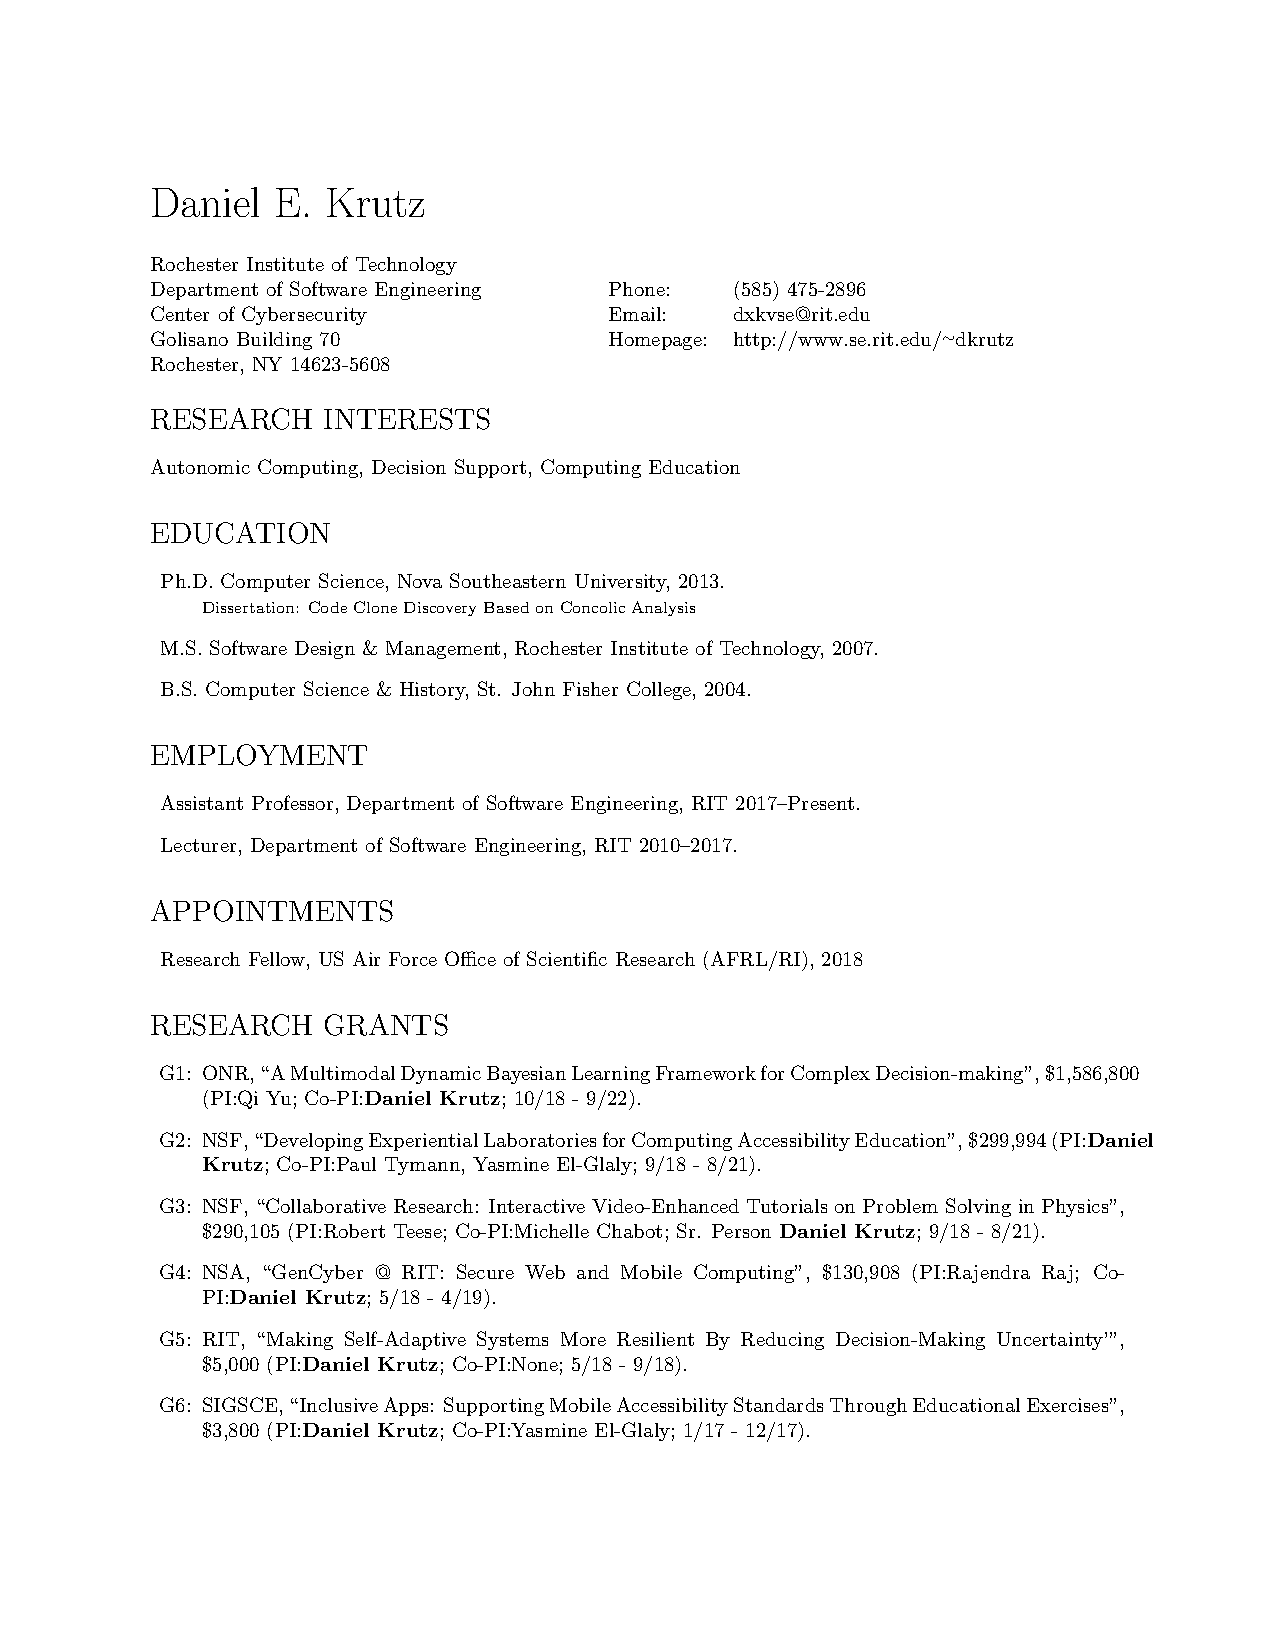
\includepdf[pages=-]{documents/cvs/Krutz_CVFull.pdf}
%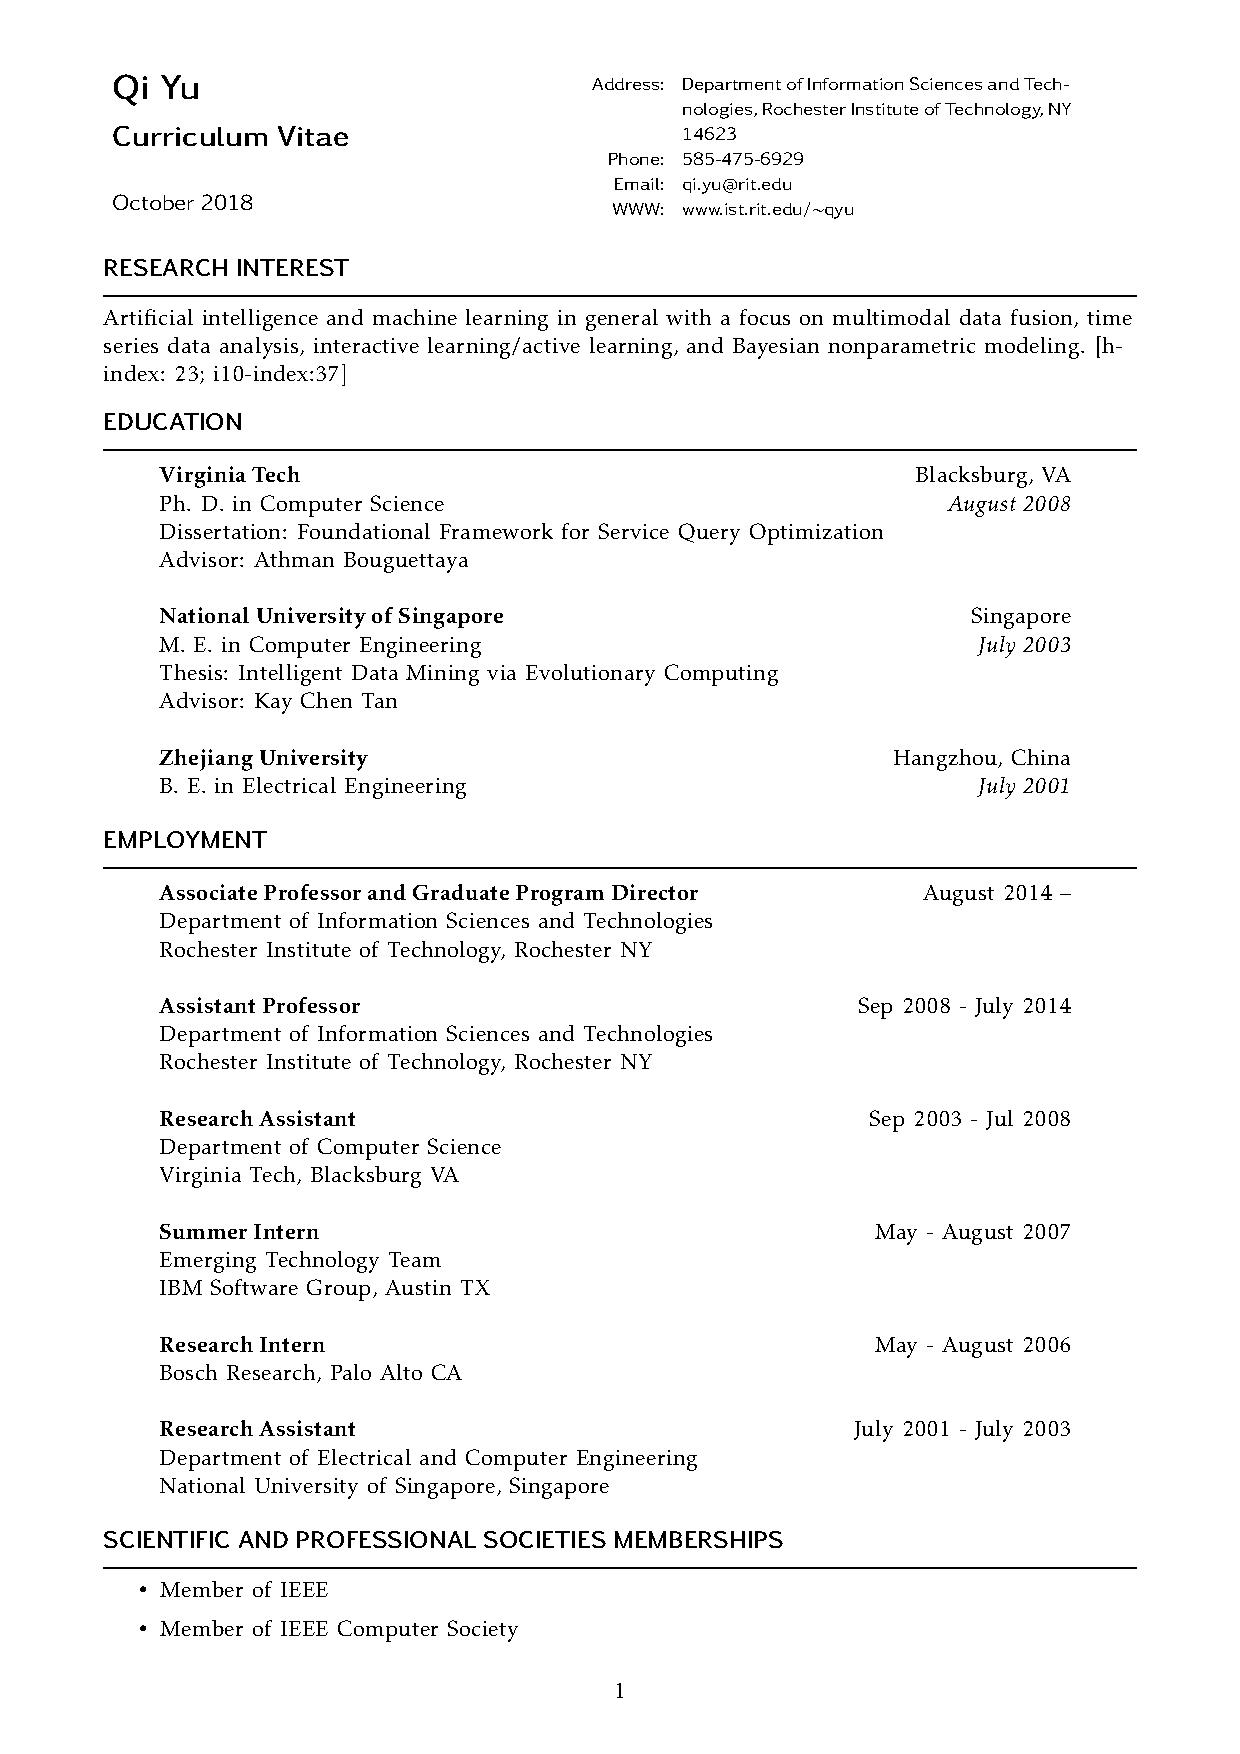
\includepdf[pages=-]{documents/cvs/Yu_CVFull.pdf}


\end{document}



% I've forwarded your document on to a few folks to see how interested they are but at first blush it appears interesting to have a method to have your AI tell you when it's likely going to make bad/erratic decisions. Please let me know if you have any questions.

%adaptation tactics—action primitives that change the system leaving it in a consistent state [13]

% [13] Shang-Wen Cheng and David Garlan. 2012. Stitch: A language for architecturebasedself-adaptation. Journal of Systems and Software 



% ? Can we add other types of volatility (from paper) into the equation



